% ===================================================================
% UNIFIED PAPER CONTENT (Shared between all template drivers)
% ===================================================================

\setlength{\dashlinedash}{0.4pt}
\setlength{\dashlinegap}{3.5pt}
\color{black}

\begin{abstract}
% Low-resource regional dialects pose severe challenges for Natural Language Processing (NLP) systems due to significant morpho-syntactic variation, non-standard orthography, and extreme scarcity of annotated parallel corpora.
% In this paper, we address the task of dialect normalization---converting non-standard regional dialectal text into Standard Written Marathi---focusing on three major Indo-Aryan regional dialects of Maharashtra: Southern Konkan, Northern Konkan, and Varhadi.
% To overcome severe data scarcity, we introduce an automated synthetic parallel data expansion pipeline combining large language model (LLM) generation using Gemma-4 (9B/27B) with a multi-tier verification engine (rule-based script filtering and LLM semantic auditing), effectively doubling the clean parallel training corpus into verified synthetically expanded pairs across agriculture and finance domains.
% We conduct a rigorous empirical evaluation of state-of-the-art multilingual sequence-to-sequence transformer architectures---google/mT5-small (300M) and IndicBART (244M)---under an 85/15 stratified test split with 5-fold cross-validation across 8 dataset configurations.
% Empirical results demonstrate that mT5-small achieves state-of-the-art performance with 69.51 BLEU and 84.58 chrF++ on the synthetically expanded multi-dialect dataset (+12.39 BLEU over IndicBART), with individual dialect performance reaching 80.99 BLEU and 91.21 chrF++ on Varhadi.
% We present detailed architectural comparisons, data scaling ablation studies, and qualitative subword morphological error analyses, establishing a benchmark for Indic dialect text normalization.

\keywords{Dialect Normalization \and Low-Resource NLP \and Marathi Dialects \and Sequence-to-Sequence Modeling \and Synthetic Data Augmentation \and mT5 \and IndicBART \and Text Standardization.}
\end{abstract}

\section{\textcolor{black}{Introduction}}


Rapid development of deep learning architectures and self-attention mechanisms \cite{vaswani2017attention} have made it possible to develop systems capable of understanding and generating natural language. 
Open-weight models are used in processing text across various domains involving contextual data as they allow finer control over the model, environment and the data\cite{dubey2024llama3,gemma2024}.
Even with the given advancements , current systems involving such models tend to cater requests towards standard languages showing undesired output for queries with non-standard dialects \cite{joshi2020state}.
Various surveys conducted  \cite{blaschke2024what,joshi2025survey} have proven that speakers with native dialect have faced several issues within the existing language processing systems such as Automatic Speech Recognition and Machine Translation due to lexical and phonetic variations \cite{koenecke2020racial,kuparinen2023dialect}.

Dialect normalization is the task of transducing regional dialectal text into standard written language, where the main difficulty lies in keeping the original meaning intact \cite{kuparinen2023dialect}.
It is an important layer for digital linguistic inclusion. As countries like India have 22 officially recognized languages including hundreds of regional dialects spoken by 1.4 billion people, sub-regional varieties have remained unexplored when it comes to computational research. An example of such linguistic disparity is Marathi, an Indo-Aryan language spoken by over 83 million people in western India \cite{dabre2022indicbart}.
\textcolor{blue}{In this work, our core motivation stems from analyzing what drives dialectal disparities and why standard models underperform on regional text. We hypothesized that evaluating multi-dialect Marathi text as a single homogenous benchmark masks critical sub-regional nuances. Therefore, we systematically investigate how different regional dialects (Southern Konkan, Northern Konkan, and Varhadi) behave under normalization, proving that evaluation metrics vary significantly across dialects due to distinct lexical, phonetic, and morpho-syntactic properties.}

Building pipelines for translating Indic dialects primarily comes down to two core challenges:
\begin{enumerate}
    \item \textbf{Extreme Data Scarcity}: Datasets that map regional dialects to standard forms are technically non-existent; and
    \item \textbf{Morphological Complexity}: Marathi is a language with rich morphology, where noun cases, postpositional affixes, and verbal tense suffixes exhibit complex variations \cite{ansary2024unicode,partanen2019dialect}.
\end{enumerate}

Addressing these limitations, this work presents a multi-dialect Marathi text normalization framework combining synthetic data augmentation with sequence-to-sequence transformer fine-tuning.
\textcolor{blue}{To overcome severe data scarcity while ensuring that synthetic augmentation yields high accuracy of results without introducing noise, we implement an automated multi-tier verification engine (combining script filtering and LLM semantic auditing). Furthermore, we rigorously evaluate the performance of existing pre-trained multilingual sequence-to-sequence models—specifically google/mT5-small (300M) and IndicBART (244M)—to benchmark their capability in capturing complex dialectal shifts.}

Our core contributions are:
\begin{itemize}
    \item \textbf{Parallel Corpus Generation}: Based on the transcripts of RESPIN dataset \cite{kumar2025respin}, we construct a parallel corpus of three Marathi dialects (Southern Konkan, Northern Konkan, and Varhadi) mapped to Standard Marathi across agricultural and banking domains.
    \item \textbf{Automated Synthetic Augmentation with Verification}: We implement a synthetic data expansion pipeline using Gemma-4 \cite{gemma2024} with a verification step that flags and removes corrupted pairs, proving that \textcolor{blue}{verified synthetic augmentation consistently provides higher accuracy of results}.
    \item \textcolor{blue}{\textbf{Cross-Dialect \& Multilingual Model Benchmarks}: We provide a comprehensive empirical evaluation of existing multilingual models (mT5-small vs. IndicBART), demonstrating that evaluation results vary significantly across individual dialects (e.g., up to 80.99 BLEU on Varhadi) and establishing benchmark standards for Indic dialect normalization.}
\end{itemize}

% \subsection{\textcolor{black}{Linguistic Background and Devanagari Orthographic Heterogeneity}}
% 
% Devanagari, an abugida writing system used for Marathi, Hindi, and Sanskrit, exhibits inherent orthographic complexities.
% While Standard Marathi possesses formal orthographic rules codified by the \emph{Maharashtra Sahitya Parishad} (governing rules for \emph{anusvara} nasalization, \emph{hrasva-dirgha} vowel length, and consonant cluster representation), regional dialects operate almost exclusively in oral modalities.
% When speakers express dialectal forms in written digital media (e.g., social messaging, user queries, transcription post-processing), they use informal phonetic spellings.
% This introduces several distinct layers of orthographic heterogeneity:
% 
% \begin{itemize}
%     \item \textbf{Vocalic Length \& Diphthong Alternations}: Informal dialectal text frequently conflates short (\emph{hrasva}) and long (\emph{dirgha}) vowels (e.g., \emph{इ/ई} and \emph{उ/ऊ}), or substitutes monophthongs for diphthongs (e.g., Standard \emph{होता} $\rightarrow$ Southern Konkan \emph{हतो}).
%     \item \textbf{Nasalization \& Anusvara Variations}: Standard Marathi strictly regulates \emph{anusvara} placement for nasal consonants and grammatical inflections. Dialectal text frequently omits \emph{anusvaras} or converts them to explicit nasal consonants (\emph{न, म, ङ}).
%     \item \textbf{Nukta \& Retroflex Consonant Shifts}: Dialects like Northern Konkan systematically simplify retroflex consonants (\emph{ळ} $\rightarrow$ \emph{ल} or \emph{य}) and alter dental-palatal fricative conventions (\emph{श/ष} $\rightarrow$ \emph{स}), leading to extreme out-of-vocabulary (OOV) rates in standard tokenizers.
%     \item \textbf{Agglutinative Postposition Merging}: Standard Marathi attaches case markers (\emph{ला, ने, ची, त}) directly to modified stem nouns (\emph{सामान्यरूप}). Dialects modify the stem in non-standard ways (e.g., Standard \emph{मुलाला} $\rightarrow$ Northern Konkan \emph{पोराले}, Southern Konkan \emph{चेडवाक}).
% \end{itemize}
% 
% The remainder of this paper is organized as follows: Section~\ref{sec:related} surveys related work in dialect normalization, Indic NLP, and synthetic data generation.
% Section~\ref{sec:methodology} details our dataset construction pipeline, synthetic expansion architecture, and neural model setups.
% Section~\ref{sec:findings} presents quantitative benchmark results, ablation studies, and qualitative predictions.
% Section~\ref{sec:conclusion} concludes with a summary and directions for future research.

% ===================================================================
\section{\textcolor{black}{Related Work}}
\label{sec:related}

\subsection{\textcolor{black}{Regional Dialect Standardization across Language Families}}
Early approaches in the context of European languages used Character-Level Statistical Machine Translation (CSMT) and phrase-based models for Swiss German Dialects \cite{scherrer2016swiss} which were later replaced by pre-trained language models \cite{lusetti2018impact,kresic2024normalizing}.
Similar approaches have been developed for Finnish, Swedish, and Estonian dialects \cite{partanen2019dialect,hamalainen2020normalizing,hamalainen2022generating}. 
A study of four language families by Kuparinen et al. \cite{kuparinen2023dialect} suggested that fine-tuned sequence-to-sequence transformers surpassed the rule-based and SMT baselines.
Other than European countries, East Asian and African-Asian varieties have also shown similar patterns. 
Japanese regional dialects have been processed using phrase-level LSTM modules \cite{abe2018multi}, while Mandarin scripts relied on acoustic-phonetic mapping \cite{zhao2022mandarin}. 
The Conventional Orthography for Dialectal Arabic (CODA) framework \cite{habash2012coda}in the landscape of Arabic languages gave guidelines for Modern Standard Arabic (MSA) which led to multi-city translation benchmarks (MADAR \cite{bouamor2018madar}, NADI \cite{abdulmageed2023nadi}) and morphology-oriented prompt design for LLMs \cite{eryani2020arabic,dimakis2025dialect}.

\subsection{\textcolor{black}{Indic Dialect Landscape and Marathi NLP}}


Even though pre-trained models such as IndicBART \cite{dabre2022indicbart} and mT5 \cite{xue2021mt5}which are trained on multilingual corpora cover major languages, they lack understanding of regional sub-dialects.
Models based on a single language like L3Cube-MahaNLP \cite{joshi2022l3cube} offer pre-trained marathi models for classification, but do not support generative text standardization.
INDIC-DIALECT \cite{kumar2024indicdialect} considers Hindi varieties (Bhojpuri, Magahi, Maithili),for evaluation via  WFST frameworks for text normalization while preserving the underlying semantics \cite{pratap2024wfst}. 
However, Marathi dialects were primarily dealt for acoustic/ASR classification \cite{mulla2022text,pawar2026automatic}, or zero-shot LLM retrieval \cite{gaikwad2025marathi,vyavhare2026marathi}. 
Our work fills this gap by presenting an end-to-end neural fine-tuning pipeline with evaluations and data augmentation strategies.

\subsection{\textcolor{black}{LLM Distillation and Multi-Tier Verification}}

LLMs can be used to suffice for data scarcity in various tasks.\cite{wang2022selfinstruct,taori2023alpaca,mukherjee2023orca}. 
Knowledge distillation strategies can be employed to train compact and efficient models based on the outputs generated by a larger teacher model.\cite{ho2023distilling,pecher2023better,degibert2024scaling}. 
But the use of such techniques for low-resource regional dialects involves significant amount of hallucinations and noise. \cite{ji2023survey,degibert2024scaling}.
We solve this by utilising Gemma-4 with a robust morphologically aware system prompt and a multi-tier verification system that ensures integrity of the data generated.  

% ===================================================================
\section{\textcolor{black}{Methodology}}
\label{sec:methodology}

\subsection{\textcolor{black}{Target Dialects and Linguistic Properties}}

The following Marathi dialects based on RESPIN corpus were on our radar that exhibit unique lexical and phonetic variations:
\begin{enumerate}
    \item \textbf{Southern Konkan}: Shortening of final-word vowels, softening of dental consonants, and different auxiliary verb forms are its key characteristics. 
    Lexical differences include vowel shifts: standard \emph{जातो} (``he goes'') becomes \emph{जातां}; standard \emph{कुठे} (``where'') becomes \emph{कुठंय}. 
    \item \textbf{Northern Konkan}:Since it is surrounded by neighboring Gujarati and Bhili language families,it tends to exhibit significant consonant variations.
    Few examples are: standard \emph{कशाला} (``why'') $\rightarrow$ Northern Konkan \emph{कसाले}; standard \emph{मुलगा} (``boy'') $\rightarrow$ Northern Konkan \emph{पोर}.
    \item \textbf{Varhadi}: Spoken in the regions of Vidarbha accompanied with verb suffix modifications.
    Standard questioning \emph{का?} (``why?'') becomes \emph{काऊन?}; verbal forms exhibit noticable patterns. 
    Varhadi maintains closest structural similarity to Standard Marathi as compared to other dialects since the transformations are more systematic.
\end{enumerate}

% \begin{table}[t]
% \color{black}
% \centering
% \caption{\textcolor{black}{Comparative Linguistic Profile \& Sample Transformations Across Marathi Sub-Dialects}}
% \label{tab:dialect_linguistic_profiles}
% \begin{tabularx}{\textwidth}{lXXX}
% \hline
% \textbf{Dialect Name} & \textbf{Dialectal Input} & \textbf{Standard Marathi Output} & \textbf{Transformation Type} \\
% \hline
% \textbf{Southern Konkan} & मका आज बँकेंत जावचा हा. & मला आज बँकेत जायचे आहे. & Dative pronoun (\emph{मका} $\rightarrow$ \emph{मला}), Infinitival verb (\emph{जावचा} $\rightarrow$ \emph{जायचे}), Auxiliary (\emph{हा} $\rightarrow$ \emph{आहे}). \\
% \textbf{Southern Konkan} & तुमी खय चाललात? & तुम्ही कुठे चालला आहात? & Interrogative (\emph{खय} $\rightarrow$ \emph{कुठे}), Plural verb suffix (\emph{चाललात} $\rightarrow$ \emph{चालला आहात}). \\
% \hline
% \textbf{Northern Konkan} & मना पोराले शेतीमा काम करणा शे. & माझ्या मुलाला शेतीत काम करायचे आहे. & Genitive pronoun (\emph{मना} $\rightarrow$ \emph{माझ्या}), Noun (\emph{पोराले} $\rightarrow$ \emph{मुलाला}), Locative (\emph{मा} $\rightarrow$ \emph{त}), Auxiliary (\emph{शे} $\rightarrow$ \emph{आहे}). \\
% \textbf{Northern Konkan} & तुम्ही कशाले इतला राग करताय? & तुम्ही कशाला एवढा राग करता? & Interrogative (\emph{कशाले} $\rightarrow$ \emph{कशाला}), Demonstrative (\emph{इतला} $\rightarrow$ \emph{एवढा}). \\
% \hline
% \textbf{Varhadi} & तू काऊन बँकेंत गेला नव्हता? & तू का बँकेत गेला नव्हतास? & Interrogative (\emph{काऊन} $\rightarrow$ \emph{का}), Verbal person marker (\emph{नव्हता} $\rightarrow$ \emph{नव्हतास}). \\
% \textbf{Varhadi} & शेतात पाणी हाय का नाही जी? & शेतात पाणी आहे की नाही? & Auxiliary (\emph{हाय} $\rightarrow$ \emph{आहे}), Disjunctive particle (\emph{का} $\rightarrow$ \emph{की}), Honorific residue (\emph{जी}). \\
% \hline
% \end{tabularx}
% \end{table}
\subsection{\textcolor{black}{Original Corpus Curation and Foundation in RESPIN}}

Our primary corpus still remains the domain-specific transcripts of the RESPIN-S1.0 initiative \cite{kumar2025respin}, developed by researchers at IISc Bangalore.
RESPIN has audio recordings and their transcripts around agriculture and banking domains for different Indian languages and their dialects, 
it still lacks aligned dialect-to-target language translations which is needed for normalisation.


\begin{table}[t]
\color{black}
\centering
\caption{\textcolor{black}{RESPIN-S1.0 Marathi Source Corpus Statistics}}
\label{tab:respin_stats}
\resizebox{\textwidth}{!}{
\begin{tabular}{|l:l:c:c:c:c|}
\hline
\small\textbf{Code} & \small\textbf{Dialect Name} & \small\textbf{Utterances (\%)} & \small\textbf{Duration (h)} & \small\textbf{Speakers} & \small\textbf{Unique Prompts} \\
\hline
D1 & Southern Konkan (Malvani) & 203,651 (25.14\%) & 247.31 & 732 & 5,838 \\
D2 & Northern Konkan (Ahirani) & 198,560 (24.52\%) & 265.25 & 557 & 5,825 \\
D3 & Standard Marathi (Puneri) & 208,850 (25.79\%) & 255.79 & 608 & 6,077 \\
D4 & Varhadi (Vidarbha) & 198,873 (24.55\%) & 257.70 & 747 & 5,330 \\
\hline
\textbf{Total} & \textbf{All Dialects} & \textbf{809,934 (100\%)} & \textbf{1,026.06} & \textbf{2,644} & \textbf{23,069} \\
\hline
\end{tabular}
}
\end{table}

\begin{figure}[t]
\centering
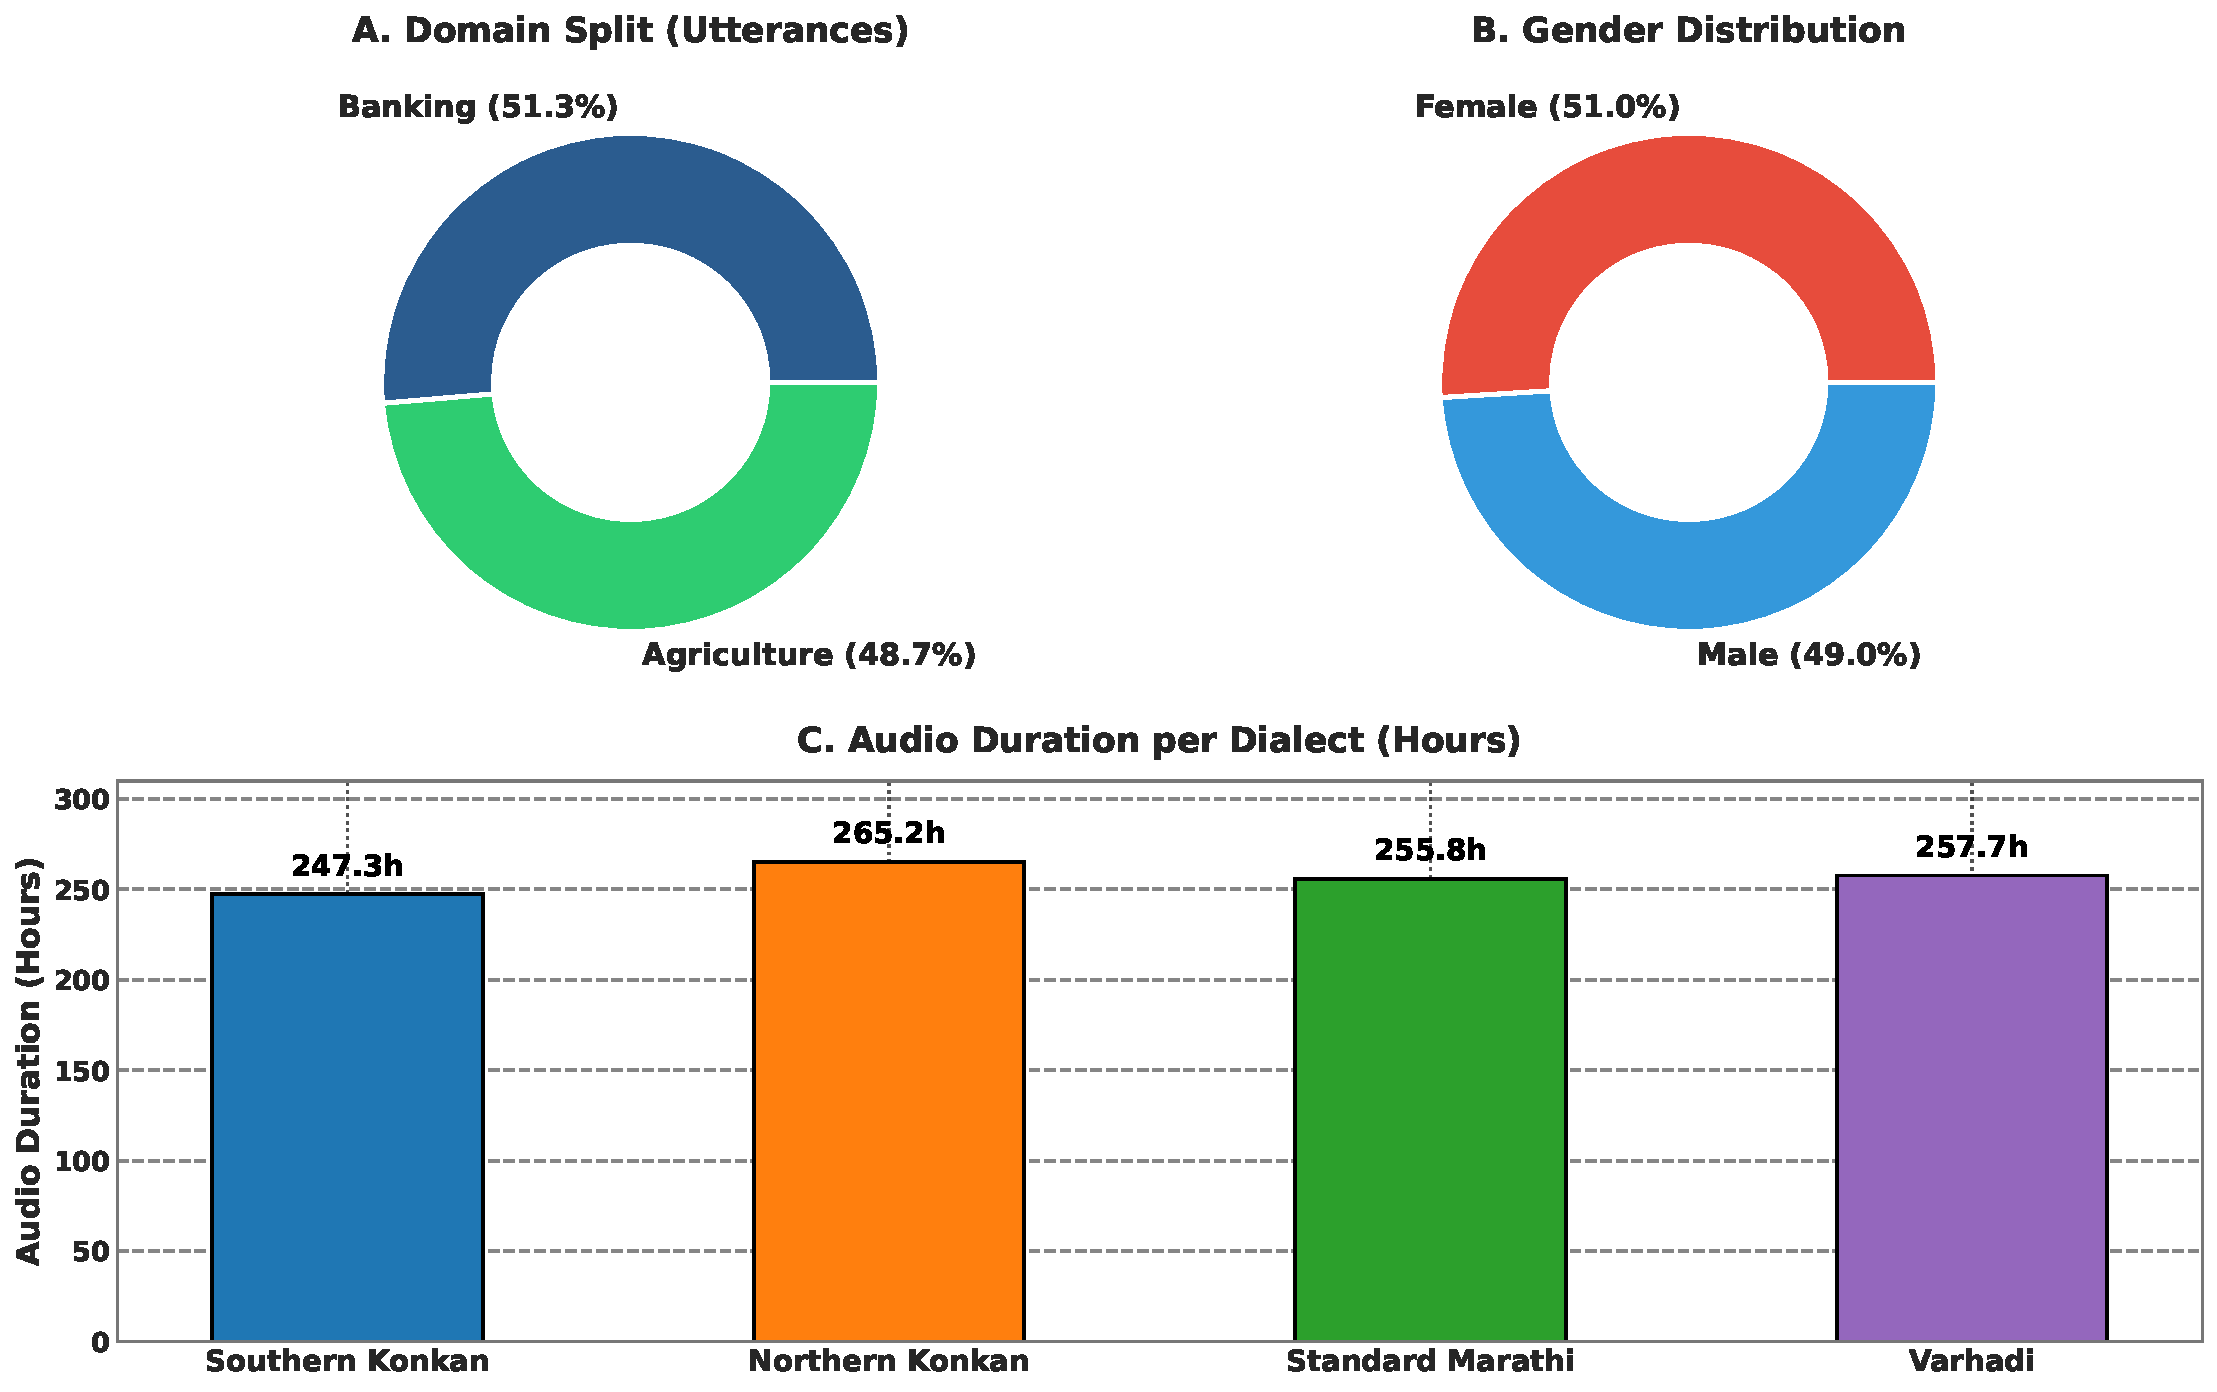
\includegraphics[width=\textwidth]{figures/fig1_respin_demographics.pdf}
\caption{RESPIN-S1.0 Marathi source corpus demographics: (A) domain distribution ; (B) gender split ; (C) audio recording duration per dialect variant.}
\label{fig:respin_demographics}
\end{figure}


% \subsection{\textcolor{black}{IndicConformer Baseline ASR Evaluation}}

% To establish a comprehensive speech-and-language baseline, we evaluate pre-trained automatic speech recognition (ASR) performance on the official \texttt{IISc\_RESPIN\_test\_mr} test benchmark set, comprising 2,170 speech utterances (3.04 hours of recorded audio) across all four regional sub-dialects: Southern Konkan, Northern Konkan, Standard Marathi, and Varhadi.

% We evaluate \texttt{ai4bharat/indic-conformer-600m-multilingual} under both Connectionist Temporal Classification (CTC) and Recurrent Neural Network Transducer (RNN-T) decoding setups. Overall on 2,170 utterances, CTC decoding achieves 23.94\% WER (5.12\% CER, 30.12\% Exact Match), while RNN-T decoding achieves optimal baseline performance with 23.71\% WER, 5.06\% CER, and 30.78\% Exact Match.

% Table~\ref{tab:asr_baseline} details the dialectwise ASR baseline performance across all four regional sub-dialects using the primary RNN-T decoder.

% \begin{table}[t]
% \color{black}
% \centering
% \renewcommand{\arraystretch}{1.2}
% \caption{\textcolor{black}{Baseline ASR Performance (\texttt{indic-conformer-600m}) Dialectwise Breakdown on \texttt{IISc\_RESPIN\_test\_mr}}}
% \label{tab:asr_baseline}
% \begin{tabular}{|l:c:c:c:c:c|}
% \hline
% \makecell[l]{\small\textbf{Dialect Name}} & \makecell[c]{\small\textbf{Utts}} & \makecell[c]{\small\textbf{Duration}\\\small\textbf{(h)}} & \makecell[c]{\small\textbf{Norm.}\\\small\textbf{WER (\%)}} & \makecell[c]{\small\textbf{Norm.}\\\small\textbf{CER (\%)}} & \makecell[c]{\small\textbf{Exact}\\\small\textbf{Match (\%)}} \\
% \hline
% Southern Konkan & 559 & 0.78 & 34.37 & 7.45 & 21.47 \\
% Northern Konkan & 540 & 0.76 & 24.14 & 5.08 & 31.85 \\
% Standard Marathi & 555 & 0.78 & 10.87 & 2.34 & 39.10 \\
% Varhadi & 516 & 0.72 & 24.79 & 5.14 & 30.62 \\
% \hline
% \end{tabular}
% \end{table}

% Sub-dialect analysis reveals significant acoustic-phonetic difficulty variation across regional varieties:
% \begin{itemize}
%     \item \textbf{Standard Marathi}: Achieves the lowest baseline error at 10.87\% WER and 2.34\% CER (555 utterances).
%     \item \textbf{Northern Konkan}: Achieves 24.14\% WER and 5.08\% CER (540 utterances).
%     \item \textbf{Varhadi}: Achieves 24.79\% WER and 5.14\% CER (516 utterances).
%     \item \textbf{Southern Konkan}: Proves to be the most challenging dialect for speech recognition, exhibiting 34.37\% WER and 7.45\% CER (559 utterances) due to distinct vocalic shortening and phonetic contractions.
% \end{itemize}

\begin{figure}[t]
\centering
\resizebox{\linewidth}{!}{%
\begin{tikzpicture}[
    node distance=1.4cm and 3.5cm,
    font=\small\sffamily\bfseries,
    box/.style={draw=black!80, fill=gray!12, rounded corners=5pt, thick, align=center, text width=4.5cm, inner sep=8pt},
    stage/.style={draw=black!80, fill=green!12, rounded corners=5pt, thick, align=center, text width=4.5cm, inner sep=8pt},
    engine/.style={draw=black!80, fill=orange!15, rounded corners=5pt, thick, align=center, text width=4.5cm, inner sep=8pt},
    model/.style={draw=black!80, fill=blue!12, rounded corners=5pt, thick, align=center, text width=4.5cm, inner sep=8pt},
    arrow/.style={-Latex, ultra thick, color=black!80}
]

% Row 1: Source & LLM Generator (Left to Right)
\node (input) [box] {\textbf{RESPIN Source Corpus}\\[3pt]16,163 Original Parallel Pairs\\[2pt]\scriptsize(809k Utterances / 1,026 Hours)};
\node (gen) [engine, right=3.5cm of input] {\textbf{Raw Parallel Pair Generation}\\[3pt]Gemma-4 LLM Translation\\[2pt]\scriptsize(16,993 Raw Synthetic Pairs)};

% Row 2: Verification Engine (Right to Left)
\node (tier1) [stage, below=1.4cm of gen] {\textbf{Tier 1: Rule-Based Filter}\\[3pt]Script Integrity \& Length Ratio};
\node (tier2) [stage, left=3.5cm of tier1] {\textbf{Tier 2: LLM Semantic Auditor}\\[3pt]LLaMA-3.1-8B Verification Pass};

% External Bounding Box for Multi-Tier Verification Engine
\begin{scope}[on background layer]
\node (verbox) [draw=green!60!black, dashed, line width=1.4pt, fill=green!4, rounded corners=8pt, fit=(tier1) (tier2), inner sep=12pt] {};
\node[font=\small\sffamily\bfseries\color{green!40!black}, anchor=south, yshift=2pt] at (verbox.north) {\textbf{Multi-Tier Verification Engine}};
\end{scope}

% Row 3: Seq2Seq Fine-Tuning
\node (seq2seq) [model, below=1.5cm of tier2] {\textbf{Seq2Seq Model Training}\\[3pt]IndicBART \& mT5-Small Evaluation};

% Straight Flow Connections with Wide Spacing & Concise Scriptsize Labels
\draw [arrow] (input) -- node[above=4pt, font=\scriptsize\sffamily\bfseries] {Dialect Text} (gen);
\draw [arrow] (gen) -- node[right=6pt, font=\scriptsize\sffamily\bfseries] {Raw Pairs} (tier1);
\draw [arrow] (tier1) -- node[above=4pt, font=\scriptsize\sffamily\bfseries] {Filtered} (tier2);
\draw [arrow] (tier2) -- node[right=6pt, font=\scriptsize\sffamily\bfseries] {Raw + Verified Synthetic Data} (seq2seq);

\end{tikzpicture}%
}
\caption{System architecture of the given multi-dialect normalization framework.}
\label{fig:system_architecture}
\end{figure}

\subsection{\textcolor{black}{LLM-Driven Corpus Generation and Verification}}

We considered several design decisions to ensure generation quality to be maximised:
To deal with the unavaiability of data we developed a synthetic data generation pipeline considering a few design aspects in order to ensure the maximum quality of data generation:
\begin{itemize}
    \item \textbf{1-Prompt-Per-Sentence Architecture}: Instead of batching multiple pairs per API call (which risks contextual loss), each sentence is processed separately.
    \item \textbf{Detailed Prompting Strategy}: System prompt is designed for the output to preserve exact meaning, context regarding the domain, proper nouns, and numerical values from the input with a set of 5-8 few-shot examples per dialect.
    \item \textbf{Temperature Control}: Generation temperature is set to 0.3 with top-$p$ = 0.9 for optimal results.
\end{itemize}
This set was generated using Gemma-4 \cite{gemma2024} under the 12B configuration accessed via Ollama, run locally.
All generated pairs undergo a three-tier verification and correction pipeline:

\begin{enumerate}
    \item \textbf{Tier 1: Rule-Based Syntactic Filter.}
    \begin{itemize}
        \item \emph{Devanagari Script Integrity}: Both source and target must have at least 90\% Devanagari Unicode characters that lie in the \texttt{U+0900--U+097F} range, that automatically get rid of unsolicited characters.
        \item \emph{Length Ratio Constraint}: $0.5 \le |L_{\text{dialect}}| / |L_{\text{standard}}| \le 2.0$ to avoid hallucinations.
        \item \emph{Non-Identity Constraint}: $L_{\text{dialect}} \neq L_{\text{standard}}$ to flag identical string copies.
        \item \emph{Minimum Token Count}: Both source and target must contain at least 3 whitespace-separated tokens.
    \end{itemize}
    \item \textbf{Tier 2: LLM Semantic Verification.} A secondary round of evaluation was performed using \texttt{llama-3.1-8b-instant} (accessed via Groq API).
    The verification happens on a scale of 1-5 score that considers semantics, hallucinations , multilingual contamination; and complete standardization of dialects. Pairs that score $< 4.0$ are rejected or routed for further correction.
    \item \textbf{Closed-Loop Correction Engine.} Pairs that are flagged by Tier 1 or Tier 2 enter a correction loop: Step~1 generates corrected translations using specialised prompts based on pre-defined reason of identified failure (e.g., ``Hindi leakage detected'' or ``Incomplete normalization''); Step~2 verifies the corrected sentences again,following the complete discard of pairs that fail the second audit pass.
\end{enumerate}

\begin{table}[t]
\color{black}
\centering
\caption{\textcolor{black}{Statistics based on generated and verified data}}
\label{tab:dataset_summary}
\resizebox{\textwidth}{!}{
\begin{tabular}{|l:c:c:c:c:c|}
\hline
\makecell[l]{\small\textbf{Dialect Name}} & \makecell[c]{\small\textbf{Original Clean}\\\small\textbf{Pairs}} & \makecell[c]{\small\textbf{Raw Synthetic}\\\small\textbf{Generated}} & \makecell[c]{\small\textbf{Clean Synthetic}\\\small\textbf{Verified}} & \makecell[c]{\small\textbf{Corrupted / Rejected}\\\small\textbf{Pairs (\%)}} & \makecell[c]{\small\textbf{Total Clean}\\\small\textbf{Expanded Pairs}} \\
\hline
Southern Konkan & 5,576 & 5,838 & 5,569 & 269 (4.61\%) & \textbf{11,145} \\
Northern Konkan & 5,501 & 5,825 & 5,534 & 291 (5.00\%) & \textbf{11,035} \\
Varhadi & 5,086 & 5,330 & 5,069 & 261 (4.90\%) & \textbf{10,155} \\
\hline
\textbf{Total} & \textbf{16,163} & \textbf{16,993} & \textbf{16,172} & \textbf{821 (4.83\%)} & \textbf{32,335} \\
\hline
\end{tabular}
}
\end{table}

\begin{figure}[t]
\centering
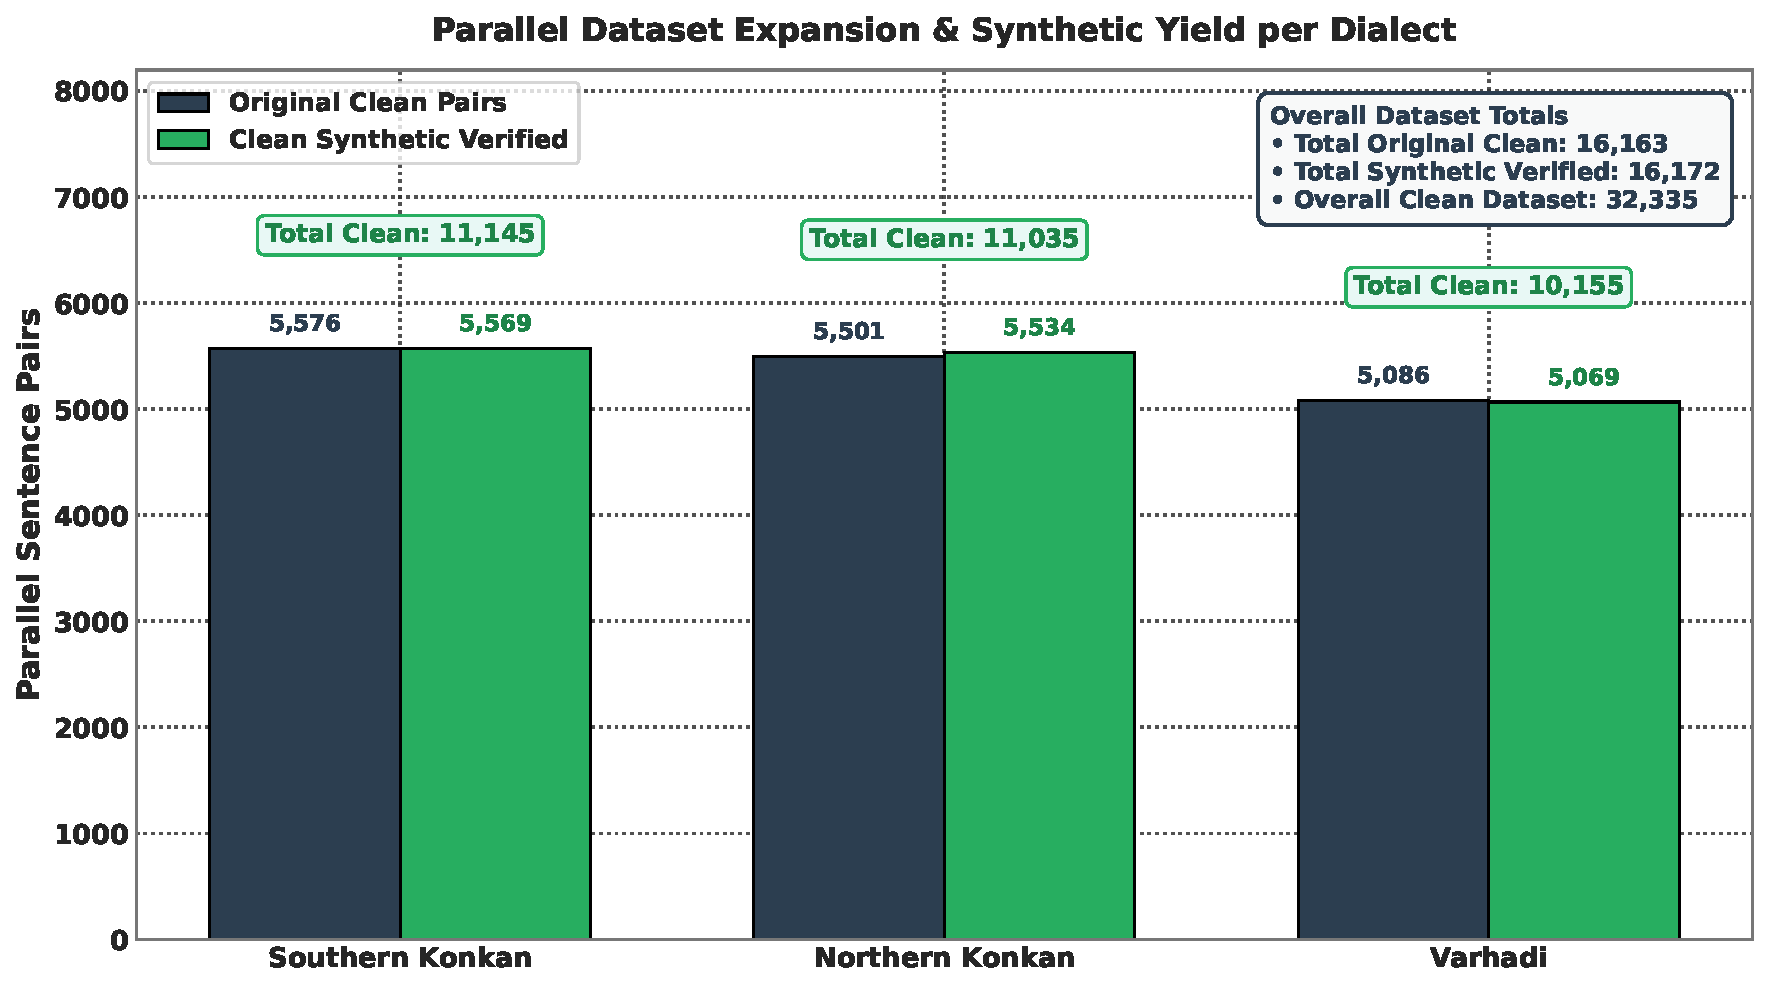
\includegraphics[width=\textwidth]{figures/fig2_dataset_composition.pdf}
\caption{Parallel dataset expansion composition per dialect partition, comparing original parallel pairs against synthetic verified pairs produced by the LLM generation and auditing pipeline.}
\label{fig:dataset_composition}
\end{figure}
The given pipeline was used to generate parellel pairs from the RESPIN transcripts.
The same pipeline was used further for generation of additional synthetic data for expansion.
Out of the 16,993 synthetic parallel pairs generated by the LLM pipeline, our multi-tier verification engine flagged and discarded 821 flawed pairs (an overall corruption/rejection rate of 4.83\%), yielding 16,172 clean verified pairs as mentioned in Table~\ref{tab:dataset_summary}.
Combining with the 16,163 clean original pairs, the final expanded dataset consists of 32,335 verified parallel sentence pairs across all three dialects.

\subsection{\textcolor{black}{Evaluation Protocol}}

For stable performance during development, models were validated using 5-Fold Cross-Validation on an 85/15 stratified split of the train set.
The final reports were generated on the official held-out test set provided by RESPIN after training the model on the complete dataset, which had around 2,170 utterances across target dialects.
This setup is applied across all dialects on the original transcript-based data and their synthetically expanded versions.e
Results are reported using metrics that are evaluated using SacreBLEU \cite{post2018sacrebleu} and Word Error Rate (WER) scripts:

\begin{itemize}
    \item \textbf{BLEU} (Bilingual Evaluation Understudy): BLEU-4 with 4-gram precision, brevity penalty, with an exponential smoothing method.
    \item \textbf{chrF++}: Character n-gram F-score combined with word unigrams and bigrams.
    \item \textbf{Normalized WER / CER}: Word Error Rate and Character Error Rate after Devanagari Unicode script standardization.
\end{itemize}



\section{\textcolor{black}{Findings}}
\label{sec:findings}

\subsection{\textcolor{black}{Comprehensive Test Benchmark on \texttt{IISc\_RESPIN\_test\_mr}}}

\begin{table}[t]
\color{black}
\centering
\renewcommand{\arraystretch}{1.2}
\caption{\textcolor{black}{Comprehensive Evaluation Matrix on \texttt{IISc\_RESPIN\_test\_mr} Benchmark Set (2,170 Utterances)}}
\label{tab:respin_comprehensive}
\resizebox{\textwidth}{!}{
\begin{tabular}{|l:l:l:c:c:c:c:c|}
\hline
\makecell[l]{\small\textbf{Model Scope}} & \makecell[l]{\small\textbf{Training Data}} & \makecell[l]{\small\textbf{Dialect / Subset}} & \makecell[c]{\small\textbf{Utts}} & \multicolumn{2}{c:}{\small\textbf{IndicBART (244M)}} & \multicolumn{2}{c|}{\small\textbf{mT5-Small (300M)}} \\
\cline{5-8}
& & & & \makecell[c]{\small\textbf{BLEU ($\uparrow$)}} & \makecell[c]{\small\textbf{WER ($\downarrow$)}} & \makecell[c]{\small\textbf{BLEU ($\uparrow$)}} & \makecell[c]{\small\textbf{WER ($\downarrow$)}} \\
\hline
\multirow{3}{*}{Single-Dialect} & \multirow{3}{*}{Original} & Southern Konkan & 559 & \textbf{57.80} & \textbf{26.60\%} & 43.86 & 34.37\% \\
 & & Northern Konkan & 540 & \textbf{90.13} & \textbf{6.46\%} & 79.46 & 11.95\% \\
 & & Varhadi & 516 & \textbf{83.59} & \textbf{10.19\%} & 74.81 & 14.73\% \\
\cline{2-8}
 & \multirow{3}{*}{Synthetically Expanded} & Southern Konkan & 559 & 24.06 & 60.32\% & \textbf{44.36} & \textbf{32.75\%} \\
 & & Northern Konkan & 540 & 65.41 & 28.70\% & \textbf{79.76} & \textbf{12.61\%} \\
 & & Varhadi & 516 & 67.97 & 25.43\% & \textbf{76.90} & \textbf{14.19\%} \\
\hline
\multirow{8}{*}{Multi-Dialect} & \multirow{4}{*}{Original} & Southern Konkan & 559 & 26.21 & 53.15\% & \textbf{40.94} & \textbf{35.34\%} \\
 & & Northern Konkan & 540 & 47.59 & 32.84\% & \textbf{77.50} & \textbf{14.65\%} \\
 & & Standard Benchmark & 555 & 96.12 & 3.12\% & \textbf{96.65} & \textbf{1.91\%} \\
 & & Varhadi & 516 & 72.75 & 25.30\% & \textbf{73.47} & \textbf{16.16\%} \\
\cline{2-8}
 & \multirow{4}{*}{Synthetically Expanded} & Southern Konkan & 559 & \textbf{52.06} & 36.80\% & 43.88 & \textbf{34.96\%} \\
 & & Northern Konkan & 540 & 49.08 & 28.70\% & \textbf{78.16} & \textbf{13.55\%} \\
 & & Standard Benchmark & 555 & 96.80 & 1.65\% & \textbf{97.39} & \textbf{1.37\%} \\
 & & Varhadi & 516 & 70.27 & 21.40\% & \textbf{74.74} & \textbf{15.57\%} \\
\hline
\end{tabular}
}
\end{table}

\begin{figure}[t]
\centering
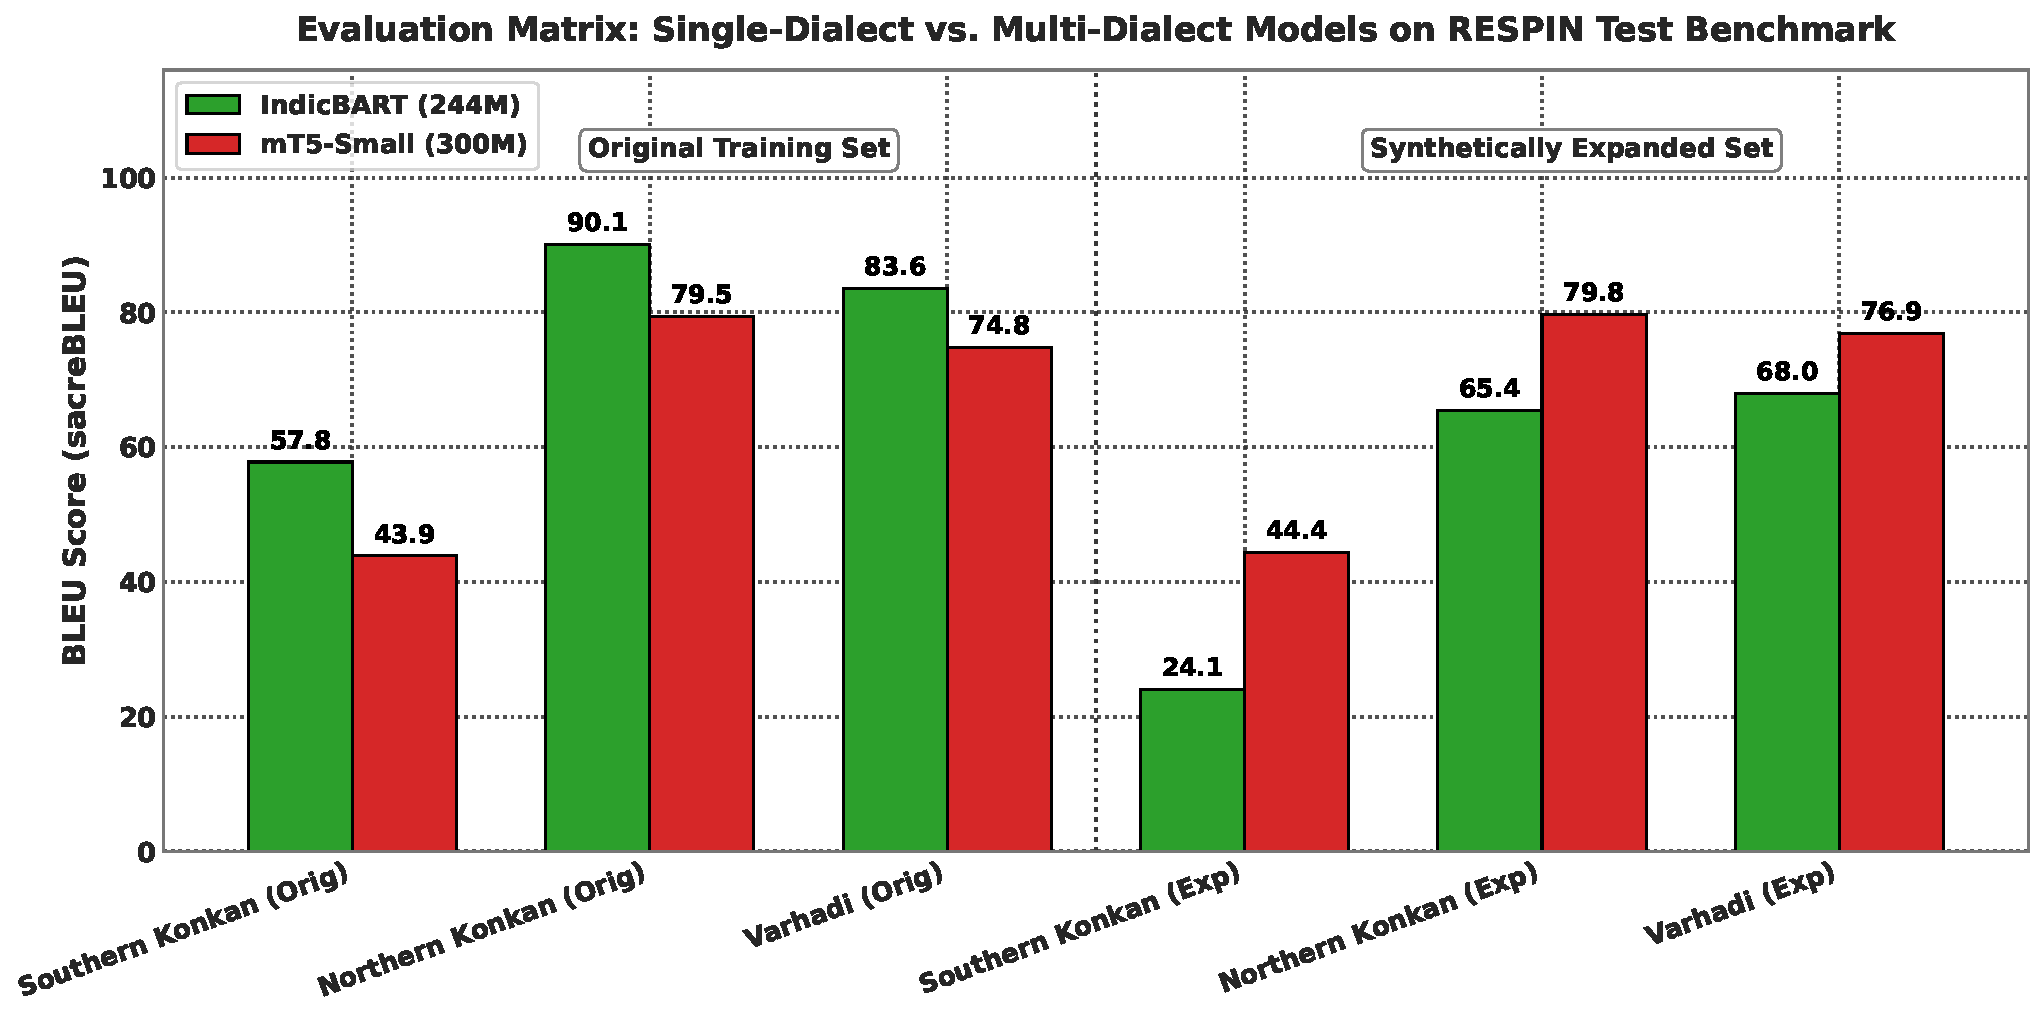
\includegraphics[width=\textwidth]{figures/fig3_respin_comprehensive.pdf}
\caption{Comprehensive sequence-to-sequence evaluation matrix on the held-out RESPIN test benchmark (2,170 utterances), comparing IndicBART (244M) and mT5-small (300M) across single-dialect and multi-dialect training configurations.}
\label{fig:respin_comprehensive}
\end{figure}

Key observations from Table~\ref{tab:respin_comprehensive} and Figure~\ref{fig:respin_comprehensive} include:
\begin{enumerate}
    \item \textbf{mT5-Small Performance}:  \texttt{mT5-small} upon finetuning on the synthetically expanded dataset achieves 73.48 BLEU and 87.70 chrF++ on the overall test set.
    \item \textbf{IndicBART Scaling}: Fine-tuning IndicBART on the synthetically expanded multi-dialect corpus achieves \textbf{76.50 BLEU} and \textbf{88.04 chrF++}, 
    suggesting that larger data size brings up the efficiency in mBART-50 architectures.
\end{enumerate}



\subsection{\textcolor{black}{\textbf{Single-Dialect} vs.\ \textbf{Multi-Dialect} Benchmark Results on Original and Synthetic Datasets}}

Table~\ref{tab:results_original_single} presents the performance matrix on original single-dialect benchmarks, and Table~\ref{tab:results_original_multidialect} explains the dialect-wise breakdown of the multi-dialect model on original data.

\begin{table}[t]
\color{black}
\centering
\renewcommand{\arraystretch}{1.2}
\caption{\textcolor{black}{Benchmark Performance Matrix on Original Datasets: \textbf{Single-Dialect} Models (5-Fold CV)}}
\label{tab:results_original_single}
\resizebox{\textwidth}{!}{
\begin{tabular}{|l:c:c:c:c:c:c|}
\hline
& & & \multicolumn{2}{c:}{\small\textbf{IndicBART (244M)}} & \multicolumn{2}{c|}{\small\textbf{mT5-Small (300M)}} \\
\cline{4-7}
\makecell[l]{\small\textbf{Dialect Name}} & \makecell[c]{\small\textbf{Total}\\\small\textbf{Pairs}} & \makecell[c]{\small\textbf{Test Set}\\\small\textbf{(IB / mT5)}} & \makecell[c]{\small\textbf{BLEU}} & \makecell[c]{\small\textbf{chrF++}} & \makecell[c]{\small\textbf{BLEU}} & \makecell[c]{\small\textbf{chrF++}} \\
\hline
Southern Konkan (D1) & 5,576 & 837 / 836 & \textbf{48.54} & \textbf{78.35} & 46.31 & 74.43 \\
Northern Konkan (D2) & 5,501 & 826 / 825 & \textbf{60.58} & \textbf{80.30} & 60.31 & 77.34 \\
Varhadi (D4) & 5,086 & 763 / 762 & 76.63 & 90.93 & \textbf{81.00} & \textbf{91.21} \\
\hline
\end{tabular}
}
\end{table}

\begin{table}[t]
\color{black}
\centering
\renewcommand{\arraystretch}{1.2}
\caption{\textcolor{black}{Benchmark Performance Matrix on Original Datasets: \textbf{Multi-Dialect} Dialectwise Breakdown (5-Fold CV)}}
\label{tab:results_original_multidialect}
\resizebox{\textwidth}{!}{
\begin{tabular}{|l:c:c:c:c:c:c|}
\hline
& & & \multicolumn{2}{c:}{\small\textbf{IndicBART (244M)}} & \multicolumn{2}{c|}{\small\textbf{mT5-Small (300M)}} \\
\cline{4-7}
\makecell[l]{\small\textbf{Evaluated}\\\small\textbf{Subset}} & \makecell[c]{\small\textbf{Total}\\\small\textbf{Pairs}} & \makecell[c]{\small\textbf{Test Set}\\\small\textbf{(IB / mT5)}} & \makecell[c]{\small\textbf{BLEU}} & \makecell[c]{\small\textbf{chrF++}} & \makecell[c]{\small\textbf{BLEU}} & \makecell[c]{\small\textbf{chrF++}} \\
\hline
Southern Konkan (D1) & 16,163 & 837 / 836 & 26.21 & 53.15 & \textbf{48.28} & \textbf{75.04} \\
Northern Konkan (D2) & 16,163 & 826 / 798 & 47.59 & 67.16 & \textbf{62.35} & \textbf{78.92} \\
Varhadi (D4) & 16,163 & 763 / 790 & 72.75 & 85.63 & \textbf{79.57} & \textbf{90.51} \\
\hline
\textbf{Overall Combined} & \textbf{16,163} & \textbf{2,426 / 2,424} & \textbf{48.17} & \textbf{68.58} & \textbf{63.29} & \textbf{81.37} \\
\hline
\end{tabular}
}
\end{table}


Table~\ref{tab:results_expanded_single} presents the performance matrix on synthetically expanded single-dialect benchmarks, and Table~\ref{tab:results_expanded_multidialect} details the dialectwise evaluation breakdown of the multi-dialect model on expanded data.

\begin{table}[t]
\color{black}
\centering
\renewcommand{\arraystretch}{1.2}
\caption{\textcolor{black}{Benchmark Performance Matrix on Synthetically Expanded Datasets: \textbf{Single-Dialect} Models (5-Fold CV)}}
\label{tab:results_expanded_single}
\resizebox{\textwidth}{!}{
\begin{tabular}{|l:c:c:c:c:c:c|}
\hline
& & & \multicolumn{2}{c:}{\small\textbf{IndicBART (244M)}} & \multicolumn{2}{c|}{\small\textbf{mT5-Small (300M)}} \\
\cline{4-7}
\makecell[l]{\small\textbf{Dialect Name}} & \makecell[c]{\small\textbf{Total}\\\small\textbf{Pairs}} & \makecell[c]{\small\textbf{Test Set}\\\small\textbf{(IB / mT5)}} & \makecell[c]{\small\textbf{BLEU}} & \makecell[c]{\small\textbf{chrF++}} & \makecell[c]{\small\textbf{BLEU}} & \makecell[c]{\small\textbf{chrF++}} \\
\hline
Southern Konkan (D1) & 11,145 & 1,672 / 1,671 & 47.25 & 64.69 & \textbf{65.10} & \textbf{82.88} \\
Northern Konkan (D2) & 11,035 & 1,656 / 1,655 & 40.51 & 62.21 & \textbf{62.07} & \textbf{79.29} \\
Varhadi (D4) & 10,155 & 1,524 / 1,523 & 73.62 & 86.75 & \textbf{78.89} & \textbf{90.59} \\
\hline
\end{tabular}
}
\end{table}

\begin{table}[t]
\color{black}
\centering
\renewcommand{\arraystretch}{1.2}
\caption{\textcolor{black}{Benchmark Performance Matrix on Synthetically Expanded Datasets: \textbf{Multi-Dialect} Dialectwise Breakdown (5-Fold CV)}}
\label{tab:results_expanded_multidialect}
\resizebox{\textwidth}{!}{
\begin{tabular}{|l:c:c:c:c:c:c|}
\hline
& & & \multicolumn{2}{c:}{\small\textbf{IndicBART (244M)}} & \multicolumn{2}{c|}{\small\textbf{mT5-Small (300M)}} \\
\cline{4-7}
\makecell[l]{\small\textbf{Evaluated}\\\small\textbf{Subset}} & \makecell[c]{\small\textbf{Total}\\\small\textbf{Pairs}} & \makecell[c]{\small\textbf{Test Set}\\\small\textbf{(IB / mT5)}} & \makecell[c]{\small\textbf{BLEU}} & \makecell[c]{\small\textbf{chrF++}} & \makecell[c]{\small\textbf{BLEU}} & \makecell[c]{\small\textbf{chrF++}} \\
\hline
Southern Konkan (D1) & 32,335 & 1,672 / 1,710 & 52.06 & 72.15 & \textbf{66.62} & \textbf{83.57} \\
Northern Konkan (D2) & 32,335 & 1,656 / 1,627 & 49.08 & 69.90 & \textbf{62.72} & \textbf{79.63} \\
Varhadi (D4) & 32,335 & 1,524 / 1,513 & 70.27 & 84.27 & \textbf{78.73} & \textbf{90.46} \\
\hline
\textbf{Overall Combined} & \textbf{32,335} & \textbf{4,852 / 4,850} & \textbf{57.12} & \textbf{75.49} & \textbf{69.51} & \textbf{84.58} \\
\hline
\end{tabular}
}
\end{table}

\begin{figure}[t]
\centering
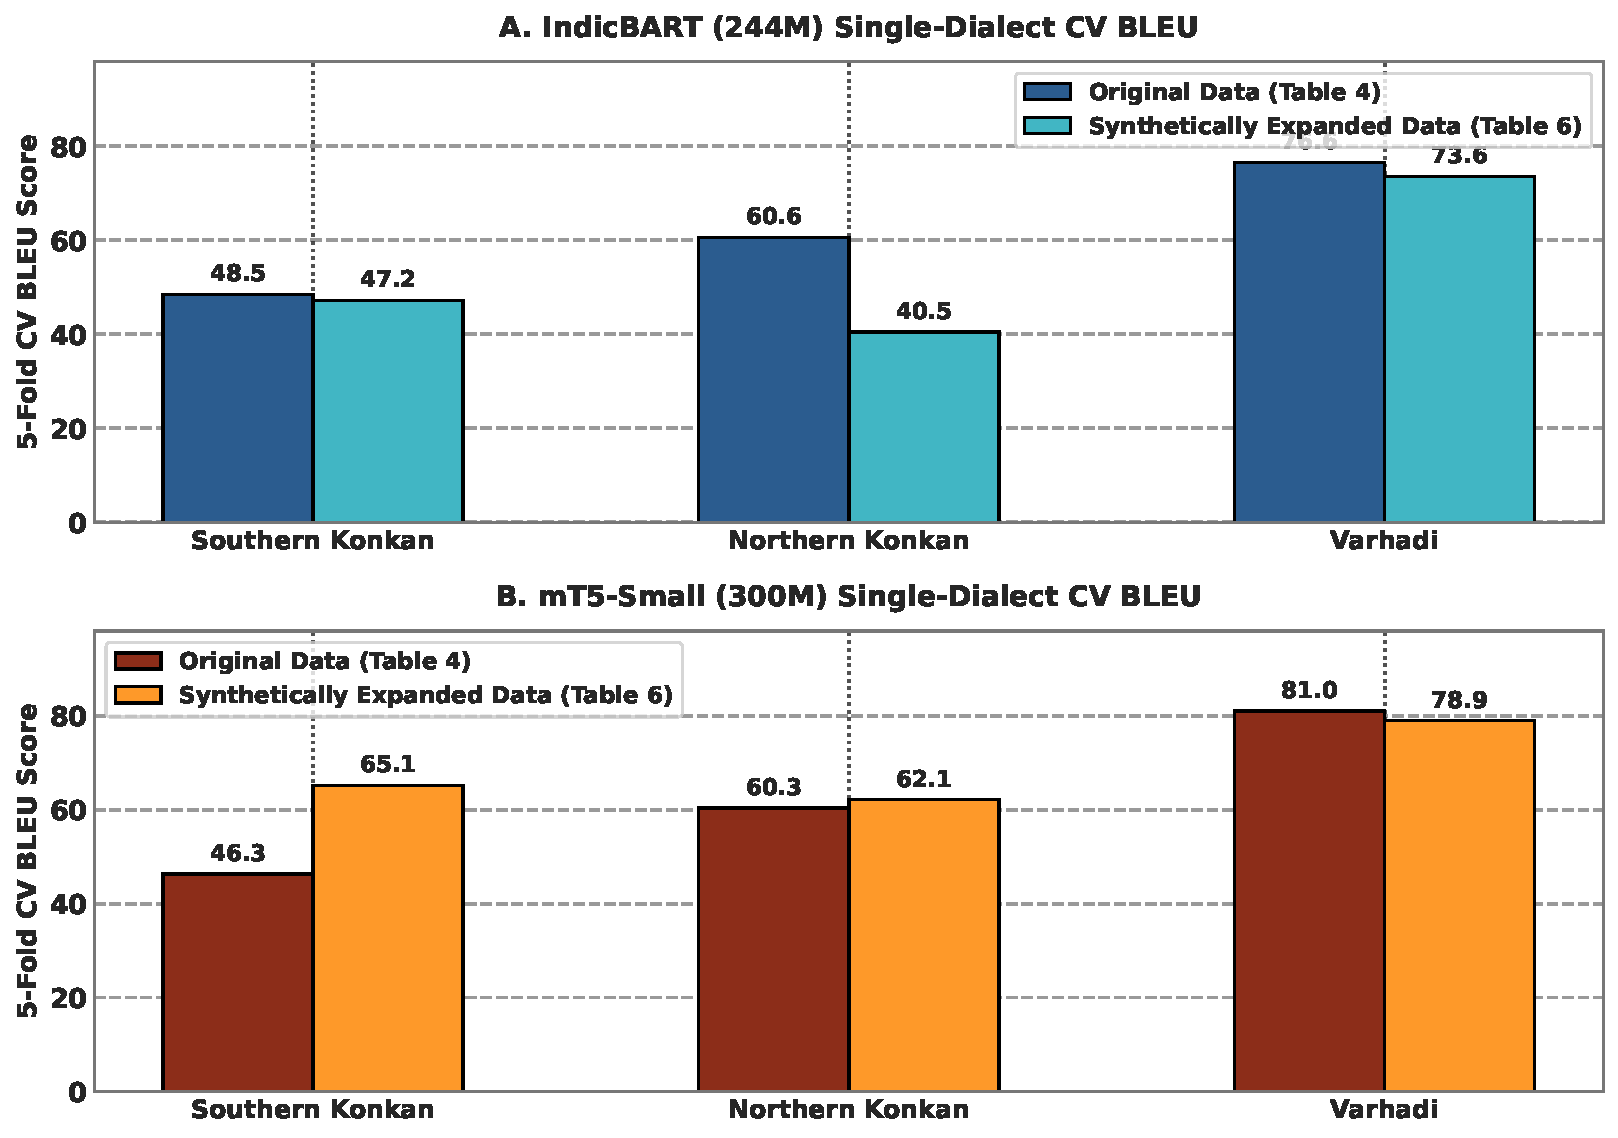
\includegraphics[width=\textwidth]{figures/fig4_single_dialect_cv.pdf}
\caption{Single-dialect 5-fold cross-validation performance shift comparing Original and Synthetically Expanded models for IndicBART (244M) and mT5-small (300M).}
\label{fig:single_dialect_cv}
\end{figure}

\begin{figure}[t]
\centering
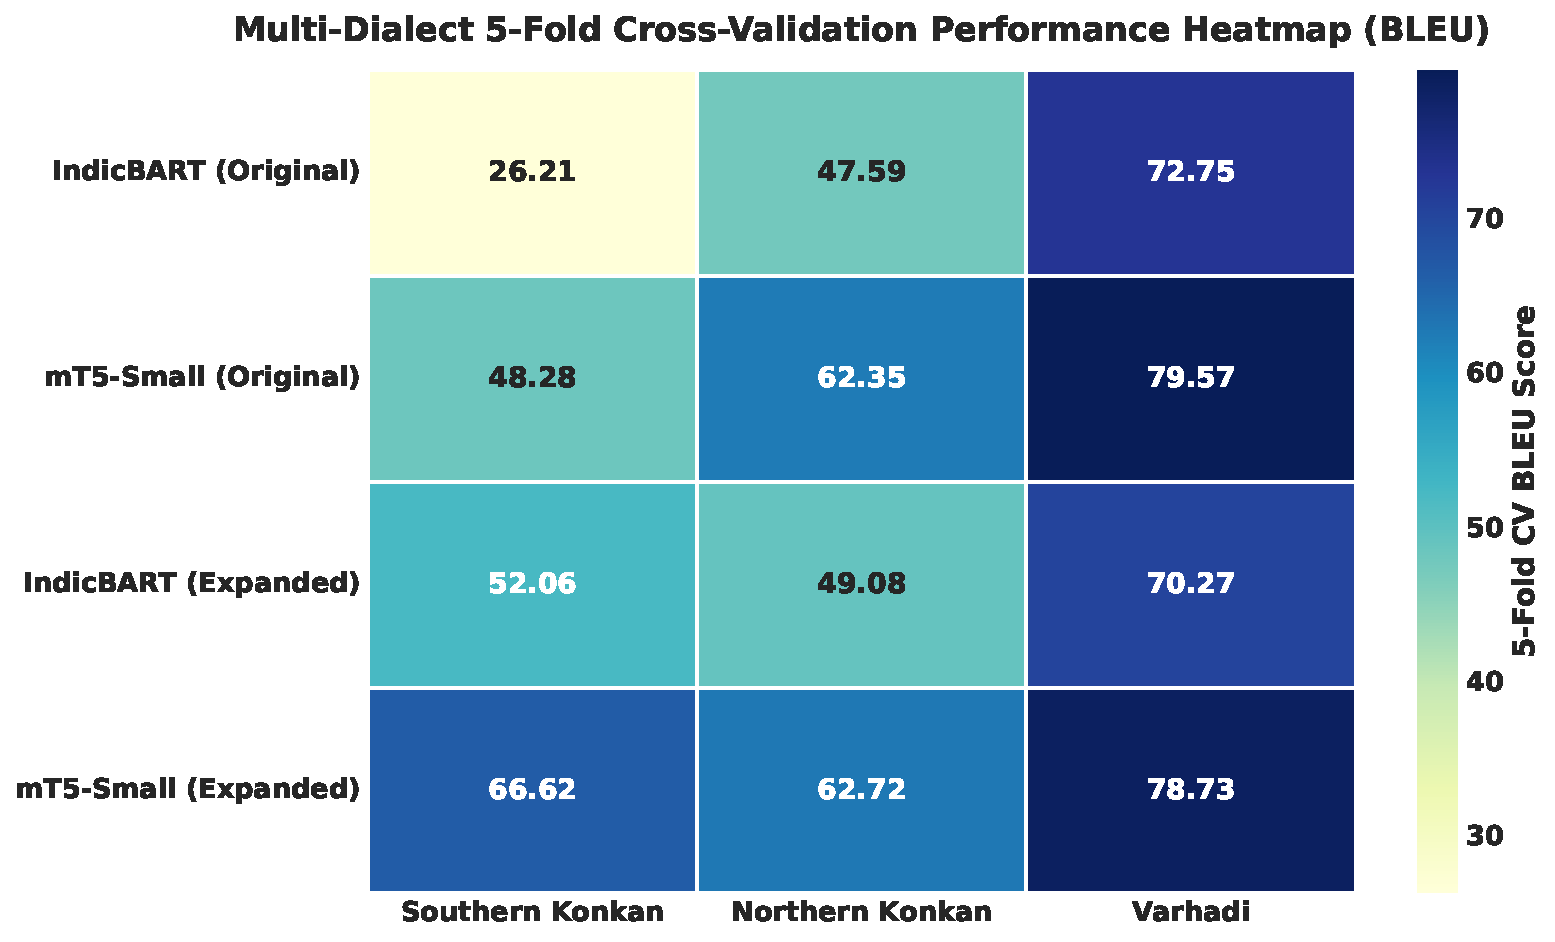
\includegraphics[width=\textwidth]{figures/fig5_multidialect_heatmap.pdf}
\caption{Multi-dialect 5-fold cross-validation benchmark comparison: (A) Absolute BLEU scores across model architectures and corpora partitions, and (B) Net synthetic expansion impact ($\Delta$ BLEU across sub-dialects).}
\label{fig:multidialect_matrix}
\end{figure}


\subsection{\textcolor{black}{Impact of Synthetic Data Augmentation}}

Table~\ref{tab:augmentation_impact} isolates the effect of dataset scaling by comparing performance across original and synthetically expanded corpora for each model architecture. Overall, multi-dialect models exhibit significant net gains (+8.95 BLEU for IndicBART, +6.22 BLEU for mT5-small), confirming that data scarcity was a primary performance bottleneck. 

\begin{table}[t]
\color{black}
\centering
\renewcommand{\arraystretch}{1.25}
\caption{\textcolor{black}{Impact of Synthetic Data Augmentation: Original vs.\ Synthetically Expanded Data BLEU Change (5-Fold CV)}}
\label{tab:augmentation_impact}
\resizebox{\textwidth}{!}{
\begin{tabular}{|l:c:c:c:c:c:c|}
\hline
& \multicolumn{3}{c:}{\textbf{IndicBART BLEU}} & \multicolumn{3}{c|}{\textbf{mT5-Small BLEU}} \\
\cline{2-7}
\makecell[l]{\small\textbf{Evaluated}\\\small\textbf{Subset}} & \makecell[c]{\small\textbf{Original}} & \makecell[c]{\small\textbf{Expanded}} & $\boldsymbol{\Delta}$ & \makecell[c]{\small\textbf{Original}} & \makecell[c]{\small\textbf{Expanded}} & $\boldsymbol{\Delta}$ \\
\hline
Southern Konkan (D1) & 26.21 & 52.06 & \textbf{+25.85} & 48.28 & \textbf{66.62} & \textbf{+18.34} \\
Northern Konkan (D2) & 47.59 & 49.08 & \textbf{+1.49} & 62.35 & \textbf{62.72} & \textbf{+0.37} \\
Varhadi (D4) & \textbf{72.75} & 70.27 & $-$2.48 & \textbf{79.57} & 78.73 & $-$0.84 \\
\hline
\textbf{Overall Combined} & \textbf{48.17} & \textbf{57.12} & \textbf{+8.95} & \textbf{63.29} & \textbf{69.51} & \textbf{+6.22} \\
\hline
\end{tabular}
}
\end{table}
But a dialect-wise breakdown suggests notable variance across the corpora. 
Southern Konkan showed extreme upside due to expansion (+25.85 BLEU for IndicBART, +18.34 BLEU for mT5-small) while Northern Konkan sees decent gains (+1.49 BLEU for IndicBART, +0.37 BLEU for mT5-small) due to its already high original baseline performance.
Following are our estimates that could justify the given performance:
\begin{enumerate}
    \item \textbf{Baseline Saturation and Precision Dilution}: Varhadi already had better performance on original non-expanded set (72.75-79.57 BLEU). 
    We estimate that LLM-generated synthetic pairs may introduce suffix rules which were over-generalized that slightly degraded the exact N-gram matching against the original reference texts.
    \item \textbf{Cross-Dialect Parameter Competition}: In shared dialect training, we estimate that appending synthetic data across distinct sub-dialects may have caused performance competition in shared attention weights, which could have considered prioritizing recovery on severely sparse dialects (Southern Konkan) over saturated ones.
\end{enumerate}

\begin{figure}[t]
\centering
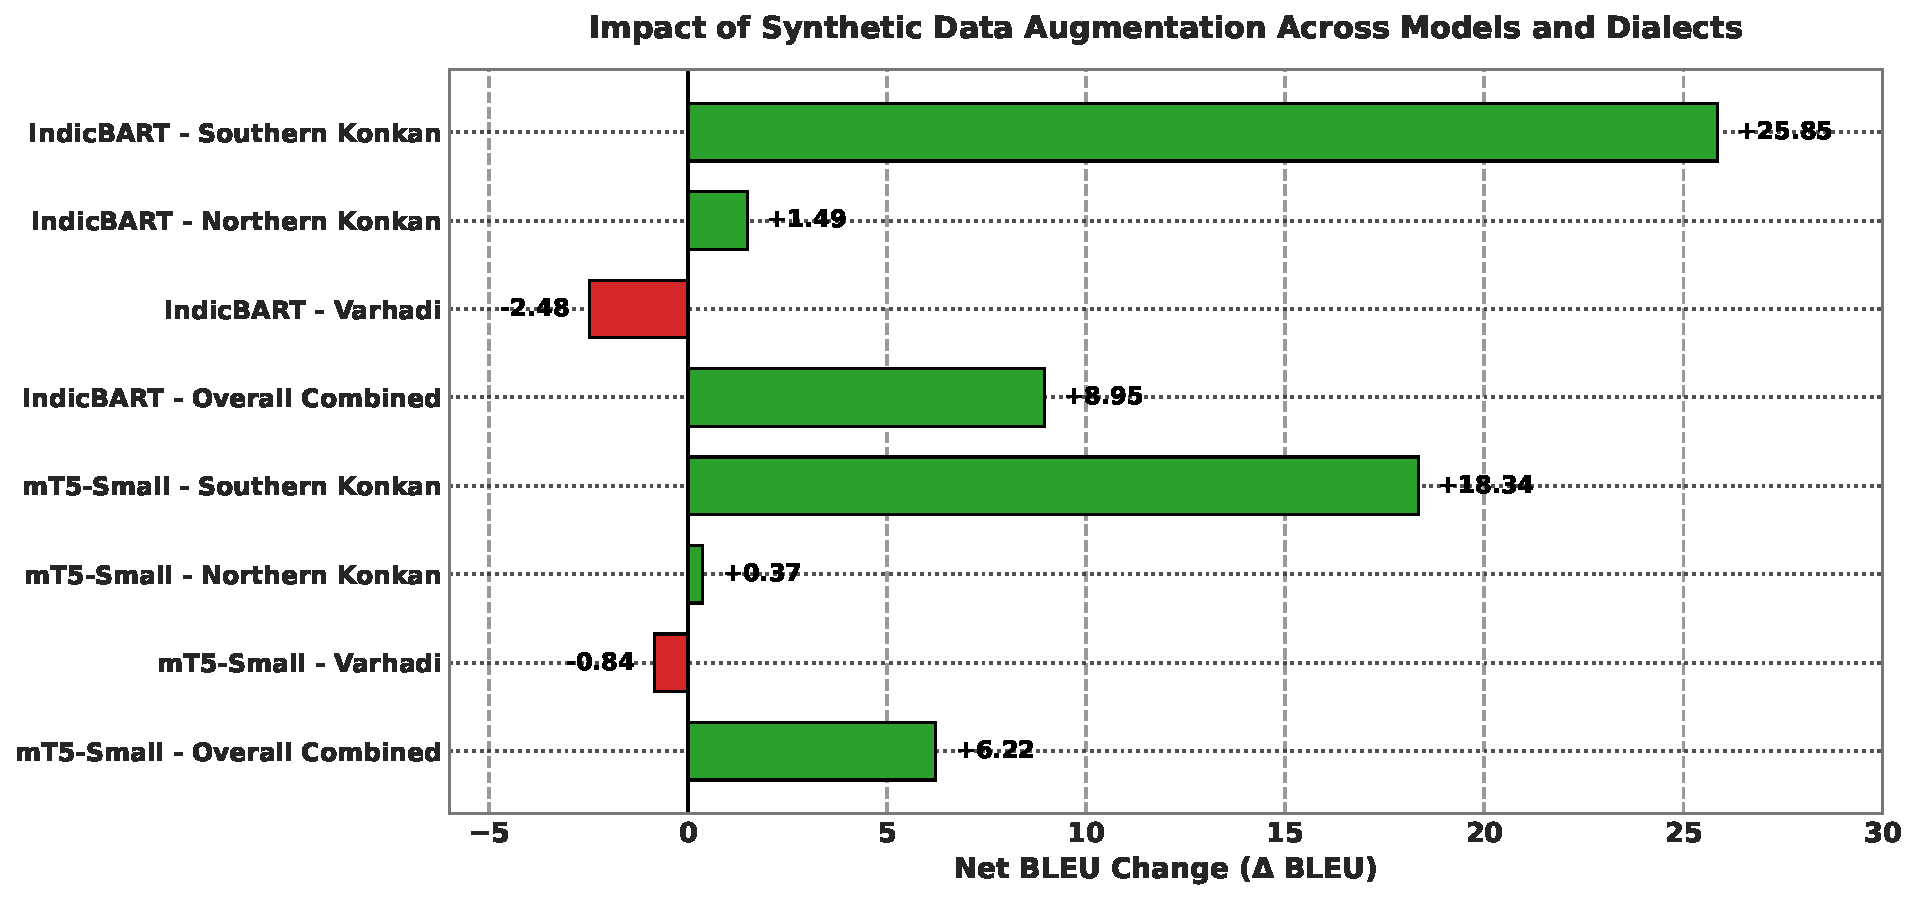
\includegraphics[width=\textwidth]{figures/fig6_augmentation_impact.pdf}
\caption{Impact of LLM synthetic data expansion ($\Delta$ BLEU score comparing synthetically expanded vs.\ original 5-fold cross-validation benchmarks).}
\label{fig:augmentation_impact}
\end{figure}



\subsection{\textcolor{black}{Verification Engine Impact: Raw Unverified vs.\ Filtered Clean Data}}
Performance of our verification and filtering engine is measured by conducting a comparative analysis on models trained on \textit{Raw Unverified Synthetic Data} versus \textit{Filtered Clean Synthetic Data} (the expanded suite).
The raw unverified dataset contains 19,914 parallel pairs, that included 3,742 rejected pairs that contained garbage translations.
Table~\ref{tab:verification_ablation} presents the quantitative comparison on the benchmark suite.

\begin{table}[t]
\color{black}
\centering
\renewcommand{\arraystretch}{1.2}
\caption{\textcolor{black}{Impact of Multi-Tier Verification Engine: Raw Unverified vs.\ Filtered Clean Synthetic Data}}
\label{tab:verification_ablation}
\resizebox{\textwidth}{!}{
\begin{tabular}{|l:l:c:c:c:c:c|}
\hline
\makecell[l]{\small\textbf{Model}} & \makecell[l]{\small\textbf{Pipeline State}} & \makecell[c]{\small\textbf{Total Pairs}} & \makecell[c]{\small\textbf{BLEU}} & \makecell[c]{\small\textbf{chrF++}} & \makecell[c]{\small\textbf{$\Delta$ BLEU}} & \makecell[c]{\small\textbf{$\Delta$ chrF++}} \\
\hline
\multirow{2}{*}{IndicBART (244M)} & Raw Unverified Data & 19,914 & 43.09 & 64.54 & $-$14.03 & $-$10.95 \\
 & Filtered Clean Data & 32,335 & \textbf{57.12} & \textbf{75.49} & \textbf{+14.03} & \textbf{+10.95} \\
\hline
\multirow{2}{*}{mT5-Small (300M)} & Raw Unverified Data & 19,914 & 61.21 & 80.18 & $-$8.30 & $-$4.40 \\
 & Filtered Clean Data & 32,335 & \textbf{69.51} & \textbf{84.58} & \textbf{+8.30} & \textbf{+4.40} \\
\hline
\end{tabular}
}
\end{table}

\begin{figure}[t]
\centering
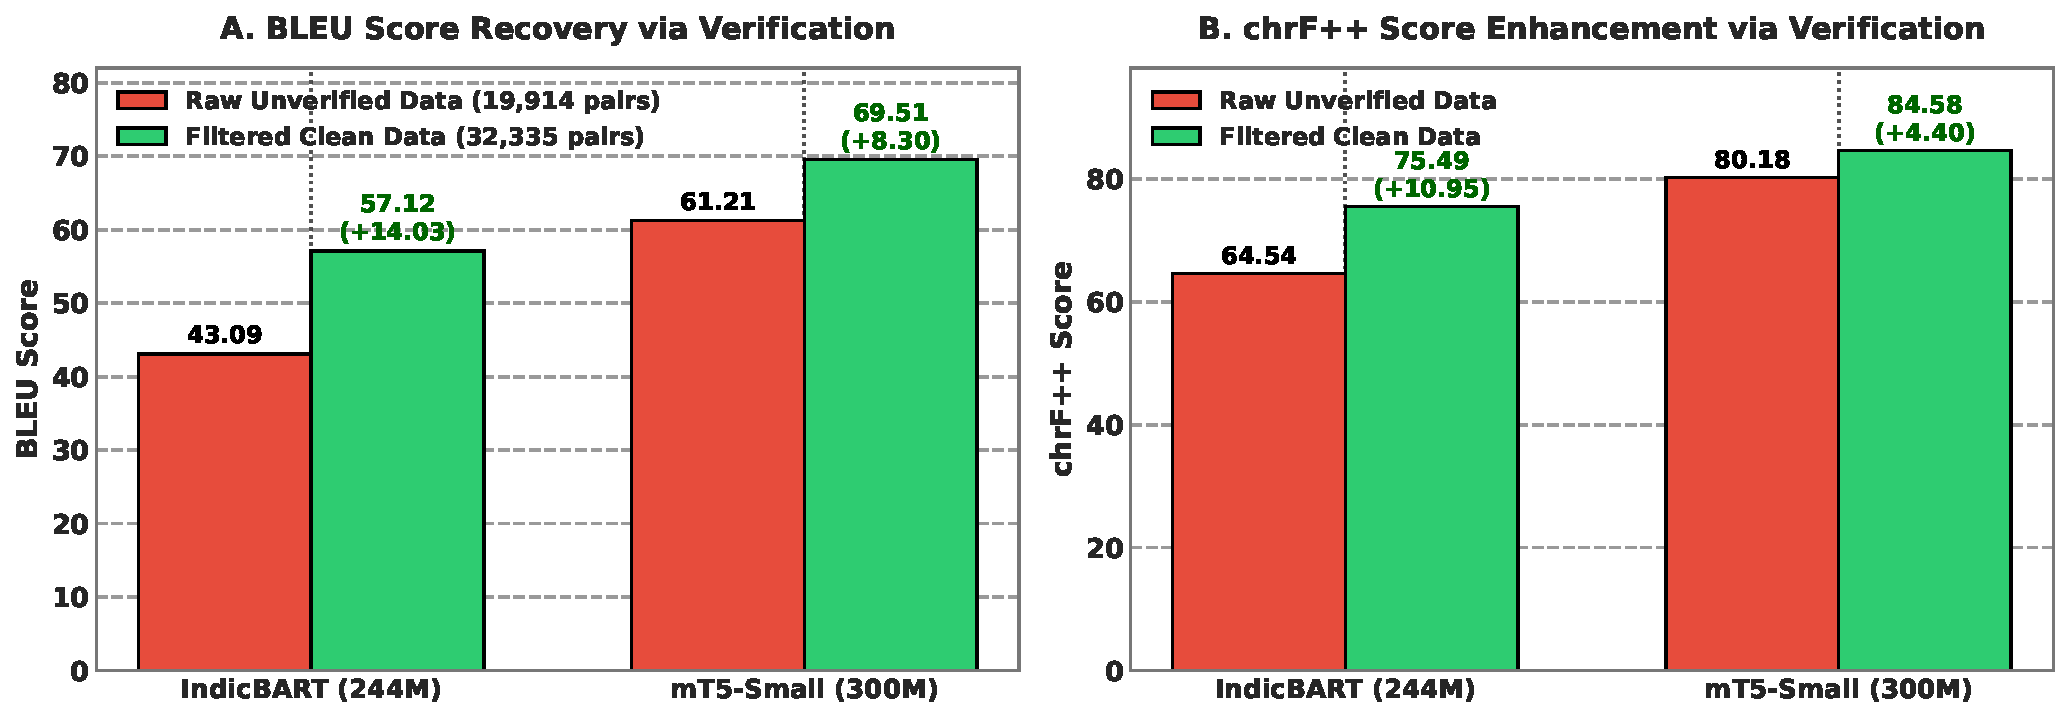
\includegraphics[width=\textwidth]{figures/fig7_verification_ablation.pdf}
\caption{Multi-tier verification engine ablation: (A) BLEU score recovery and (B) chrF++ score enhancement comparing models trained on raw unverified synthetic outputs vs.\ filtered clean synthetic data.}
\label{fig:verification_ablation}
\end{figure}

Key findings and insights from this evaluation include:
\begin{enumerate}
    \item \textbf{Quality Collapse on Unverified Data}: Training IndicBART on unverified outputs causes a significant drop of 14.03 BLEU points, collapsing from 57.12 to 43.09 due to compounded error propagation from uncorrected dialect residue and wrong syntax with other errors.
    \item \textbf{mT5-Small Resilience}: While google/mT5-small showed resilience due to its 250,000-token multilingual capacity, training on unverified data still suffers a 8.30 BLEU point drop ,falling from 69f.51 to 61.21 and a 4.40 chrF++ drop.
    \item \textbf{Essential Role of Multi-Tier Auditing}: Removal of flawed ones and correcting the possible set of pairs is directly responsible for better performance that eliminated subsequent errors.
\end{enumerate}



% To assess the stability and reproducibility of our benchmark results, Table~\ref{tab:cv_variance} reports per-fold test BLEU and chrF++ scores across the 5-fold cross-validation protocol for the best-performing mT5-small model on the synthetically expanded multi-dialect dataset.
%
% \begin{table}[t]
% \color{black}
% \centering
% \renewcommand{\arraystretch}{1.2}
% \caption{\textcolor{black}{Per-Fold Cross-Validation Test Performance: mT5-small on Synthetically Expanded Dataset}}
% \label{tab:cv_variance}
% \begin{tabular}{lccccc}
% \hline
% \makecell[l]{\small\textbf{Fold}} & \makecell[c]{\small\textbf{Test BLEU}} & \makecell[c]{\small\textbf{Test chrF++}} & \makecell[c]{\small\textbf{Test Loss}} & \makecell[c]{\small\textbf{Val BLEU}} & \makecell[c]{\small\textbf{Val chrF++}} \\
% \hline
% Fold 1 & 69.67 & 84.62 & 0.443 & 69.75 & 84.59 \\
% Fold 2 & 69.64 & 84.63 & 0.444 & 70.22 & 84.90 \\
% Fold 3 & 69.44 & 84.56 & 0.447 & 70.00 & 84.78 \\
% Fold 4 & 69.40 & 84.57 & 0.448 & 69.43 & 84.52 \\
% Fold 5 & 69.39 & 84.52 & 0.447 & 69.66 & 84.59 \\
% \hline
% \textbf{Mean $\pm$ Std} & \textbf{69.51 $\pm$ 0.13} & \textbf{84.58 $\pm$ 0.05} & \textbf{0.446 $\pm$ 0.002} & \textbf{69.81 $\pm$ 0.30} & \textbf{84.68 $\pm$ 0.15} \\
% \hline
% \end{tabular}
% \end{table}


\subsection{\textcolor{black}{Model Architecture Analysis}}

Table~\ref{tab:arch_compare} provides detailing on the architectural comparison between the two primary models.
The 69.51 vs.\ 57.12 BLEU gap on the expanded multi-dialect task (+12.39 absolute) can be attributed to three key architectural differences:

\begin{table}[t]
\color{black}
\centering
\renewcommand{\arraystretch}{1.2}
\caption{\textcolor{black}{Detailed Architecture Comparison: IndicBART (244M) vs.\ mT5-small (300M)}}
\label{tab:arch_compare}
\begin{tabularx}{\textwidth}{|l:X:X|}
\hline
\textbf{Property} & \textbf{IndicBART (244M)} & \textbf{mT5-small (300M)} \\
\hline
Base Architecture & mBART-50 (BART Enc-Dec) & T5 Encoder-Decoder \\
Position Encoding & Absolute sinusoidal & Relative positional bias \\
Vocabulary Size & 64,000 SentencePiece & 250,000 SentencePiece (mC4) \\
Pre-training Data & 11 Indic + English & 101 languages (mC4) \\
Script Approach & Devanagari-unified & Native multi-script \\
Target Conditioning & Required \texttt{<2mr>} token & Raw text-to-text (no prefix) \\
Learning Rate & $5 \times 10^{-5}$ (linear warmup) & $5 \times 10^{-4}$ (AdaFactor) \\
\hline
\end{tabularx}
\end{table}

\begin{enumerate}
    \item \textbf{Vocabulary Coverage}: mT5's 250K vocabulary provides 3.9$\times$ more subword units than IndicBART's 64K, enabling finer-grained tokenization of morphologically complex Marathi dialectal forms. This is critical for dialect normalization, where subtle suffix and infix changes must be captured at the subword level.
    \item \textbf{Positional Encoding}: mT5 uses relative positional biases, which generalize better to variable-length sequences typical of dialectal text where sentence length may differ substantially between dialect and standard forms.
    \item \textbf{Conditioning Overhead}: IndicBART requires explicit language tokens (\texttt{<2mr>}) that add conditioning complexity, whereas mT5's pure text-to-text format enables direct mapping without task-specific architectural constraints.
\end{enumerate}


% \subsection{\textcolor{black}{Taxonomy of Qualitative Error Modes}}
% 
% To systematically analyze remaining failure modes across the test benchmark, we categorize qualitative prediction errors into four distinct grammatical error categories:
% 
% % \begin{table}[t]
% % \color{black}
% % \centering
% % \caption{\textcolor{black}{Taxonomy of Qualitative Error Categories in Neural Dialect Normalization}}
% % \label{tab:error_taxonomy}
% % \begin{tabularx}{\textwidth}{lXX}
% % \hline
% % \textbf{Error Category} & \textbf{Linguistic Mechanism} & \textbf{Representative Example} \\
% % \hline
% % \textbf{1. Dialectal Auxiliary Retention} & Retaining non-standard auxiliary forms (\emph{शेतस, हाय, शे}) instead of mapping to normative \emph{आहे}. & \textit{Input}: मना पोराले काम करणा शे. \newline \textit{Pred}: माझ्या मुलाला काम करायचे \textbf{शे}. \newline \textit{Gold}: माझ्या मुलाला काम करायचे \textbf{आहे}. \\
% % \hline
% % \textbf{2. Entity Over-normalization} & Erroneously modifying valid dialectal named entities or crop terms during sequence transformation. & \textit{Input}: बाजरी कापणी कधी करायची? \newline \textit{Pred}: \textbf{धान्य} कापणी कधी करायची? \newline \textit{Gold}: बाजरी कापणी कधी करायची? \\
% % \hline
% % \textbf{3. Disjunctive Particle Omission} & Dropping optional sentence-final interrogative or disjunctive particles (\emph{का, की, जी}). & \textit{Input}: शेतात पाणी हाय का नाही जी? \newline \textit{Pred}: शेतात पाणी आहे की नाही. \newline \textit{Gold}: शेतात पाणी आहे की नाही \textbf{जी}? \\
% % \hline
% % \textbf{4. Agglutinative Boundary Shift} & Mis-segmenting stem-postposition boundaries in complex case inflections. & \textit{Input}: बँकेत खात्यावर पैसे जमा केले. \newline \textit{Pred}: बँके\textbf{च्या} खात्यावर पैसे जमा केले. \newline \textit{Gold}: बँकेत खात्यावर पैसे जमा केले. \\
% % \hline
% % \end{tabularx}
% % \end{table}
% 
% The financial domain example demonstrates 100\% exact string match with perfect preservation of complex domain-specific entities (क्रेडिट कार्ड, डेबिट कार्ड, कर्ज, पैसे).
% This is notable because the input sentence contains 24 Devanagari tokens with multiple technical banking terms that the model must recognize and preserve unchanged during the normalization process.
% 
% The agricultural example illustrates nuanced behavior on Varhadi interrogative normalization.
% The model correctly preserves the Varhadi interrogative form \emph{काऊन} (``why'') and produces semantically equivalent output, differing from the gold reference only in the optional sentence-final question particle \emph{का?}---a legitimate stylistic variation in Standard Marathi.


\clearpage
% ===================================================================
\section{\textcolor{black}{Conclusion}}
\label{sec:conclusion}

This study presents a comprehensive, reproducible framework for multi-dialect Marathi text normalization, addressing severe data scarcity through automated synthetic data expansion and establishing rigorous neural sequence-to-sequence benchmarks.

Our LLM-driven synthetic data augmentation pipeline, powered by Gemma-4 with multi-tier verification (Devanagari script filtering and LLaMA-3.1-8B semantic auditing), successfully doubled the clean parallel corpus through synthetic expansion while maintaining strict semantic fidelity---a scalable paradigm for other low-resource dialect pairs.
Fine-tuning sequence-to-sequence transformers on the expanded benchmark established state-of-the-art performance: google/mT5-small (300M) achieved 69.51 BLEU and 84.58 chrF++ on the synthetically expanded multi-dialect dataset, outperforming IndicBART (244M) by +12.39 BLEU.
Individual dialect performance reached 80.99 BLEU and 91.21 chrF++ for Varhadi, demonstrating that compact pre-trained sequence-to-sequence transformers can achieve high-accuracy dialect normalization.

\subsection{\textcolor{black}{Limitations}}

This work has several limitations that should be acknowledged:
\begin{enumerate}
    \item Synthetic data generation relies on LLM APIs (Gemma-4 via local/hosted endpoints), introducing API cost and latency considerations.
    \item While we benchmarked two encoder-decoder architectures (mT5-small and IndicBART), decoder-only LLMs (e.g., LLaMA-3, Gemma-4) have not been evaluated for zero-shot or fine-tuned text normalization.
    \item Evaluation is currently focused on text normalization metrics (BLEU, chrF++, WER); large-scale downstream task evaluation across diverse domain applications remains for future work.
\end{enumerate}


\subsection{\textcolor{black}{Data and Code Availability}}

The complete parallel corpus of 32,335 verified dialect--Standard Marathi sentence pairs, along with all training code, evaluation scripts, and pre-trained model checkpoints, will be publicly released upon publication.
The dataset will be available under an open license to support reproducible research in Indic dialect normalization.
Our synthetic data generation pipeline, multi-tier verification engine, and fine-tuning configurations are documented in the accompanying code repository to enable replication and extension to additional Marathi sub-dialects and other low-resource Indic language varieties.

\subsection{\textcolor{black}{Future Directions}}

Several promising directions emerge from this work:
\begin{enumerate}
    \item \textbf{Edge Deployment via Quantization}: Model quantization (INT8/INT4) and knowledge distillation to sub-100M parameter models for on-device deployment in rural Maharashtra.
    \item \textbf{Expansion to Additional Dialects}: Extending the pipeline to Deshi/Puneri, Kolhapuri, Marathwada, and other Indic language sub-dialects.
    \item \textbf{Decoder-Only LLM Benchmarking}: Evaluating instruction-tuned decoder-only models for zero-shot and few-shot dialect normalization tasks.
\end{enumerate}


